\mychapter{Resultat}
\label{chap:resultat}
Notera att tiden som visas i tabellerna är i sekunder och är ett medelvärde av 25 enskilda
krypteringsomgångar för varje nyckel och varje körläge.
Det råa data värdena från hela undersökningen
går att se i bilaga \ref{app:raw-data-mode-picture-test}, \ref{app:raw-data-keylength} \& \ref{app:raw-data-mode}.

\section{Nyckellängdstest}
\label{sec:nyckellangd}

\begin{table}[H]
    \centering
    \begin{tabular}{ |c|c|c|c| }
      \multicolumn{4}{c}{\bfseries{Resultat Tid (s)}} \\
      \hline
      & \bfseries{ECB - 128bit} & \bfseries{ECB - 192bit} & \bfseries{ECB - 256bit} \\
      \hline
      \bfseries{Maxvärde} & 21,7096068999963 & 25,3103521000012 & 29,2763711000007 \\
      \hline
      \bfseries{Minvärde} & 20,8357139000000 & 24,8878867999956 & 29,0315928999989 \\
      \hline
      \bfseries{Medelvärde} & 21,0575238279998 & 25,01450157200015 & 29,17758371600008 \\
      \hline
    \end{tabular}
\end{table}

\begin{table}[H]
  \centering
  \begin{tabular}{ |c|c| }
    \multicolumn{2}{c}{\bfseries{Procentuell skillnad (medelvärde)}} \\
    \hline
    \bfseries{ECB - 128bit \& 192bit} & 18,8\% \\
    \hline
    \bfseries{ECB - 192bit \& 256bit} & 16,6\% \\
    \hline
    \bfseries{ECB - 128bit \& 256bit} & 27,8\% \\
    \hline
  \end{tabular}
\end{table}

\section{Körlägestest}
\label{sec:korlages}

\begin{table}[H]
    \centering
    \begin{tabular}{ |c|c|c|c| }
      \multicolumn{4}{c}{\bfseries{Resultat Tid (s)}} \\
      \hline
      & \bfseries{ECB - 128bit} & \bfseries{CBC - 128bit} & \bfseries{OFB - 128bit} \\
      \hline
      \bfseries{Maxvärde} & 21,0857602999968 & 20,9346826999972 & 20,8816630000001 \\
      \hline
      \bfseries{Minvärde} & 20,8010089999952 & 20,8505676999994 & 20,7675767999972 \\
      \hline
      \bfseries{Medelvärde} & 20.82165230000013 & 20.885069635999972 & 20.89562146799988 \\
      \hline
    \end{tabular}
\end{table}

\begin{table}[H]
  \centering
  \begin{tabular}{ |c|c| }
    \multicolumn{2}{c}{\bfseries{Procentuell skillnad (medelvärde)}} \\
    \hline
    \bfseries{ECB - 128bit \& CBC - 128bit} & 0,3\% \\
    \hline
    \bfseries{CBC - 128bit \& OFB - 128bit} & 0,1\% \\
    \hline
    \bfseries{ECB - 128bit \& OFB - 128bit} & 0,4\% \\
    \hline
  \end{tabular}
\end{table}

\section{Krypteringstest}
\label{sec:krypterings-test}

\begin{figure}[H]
      \centering
    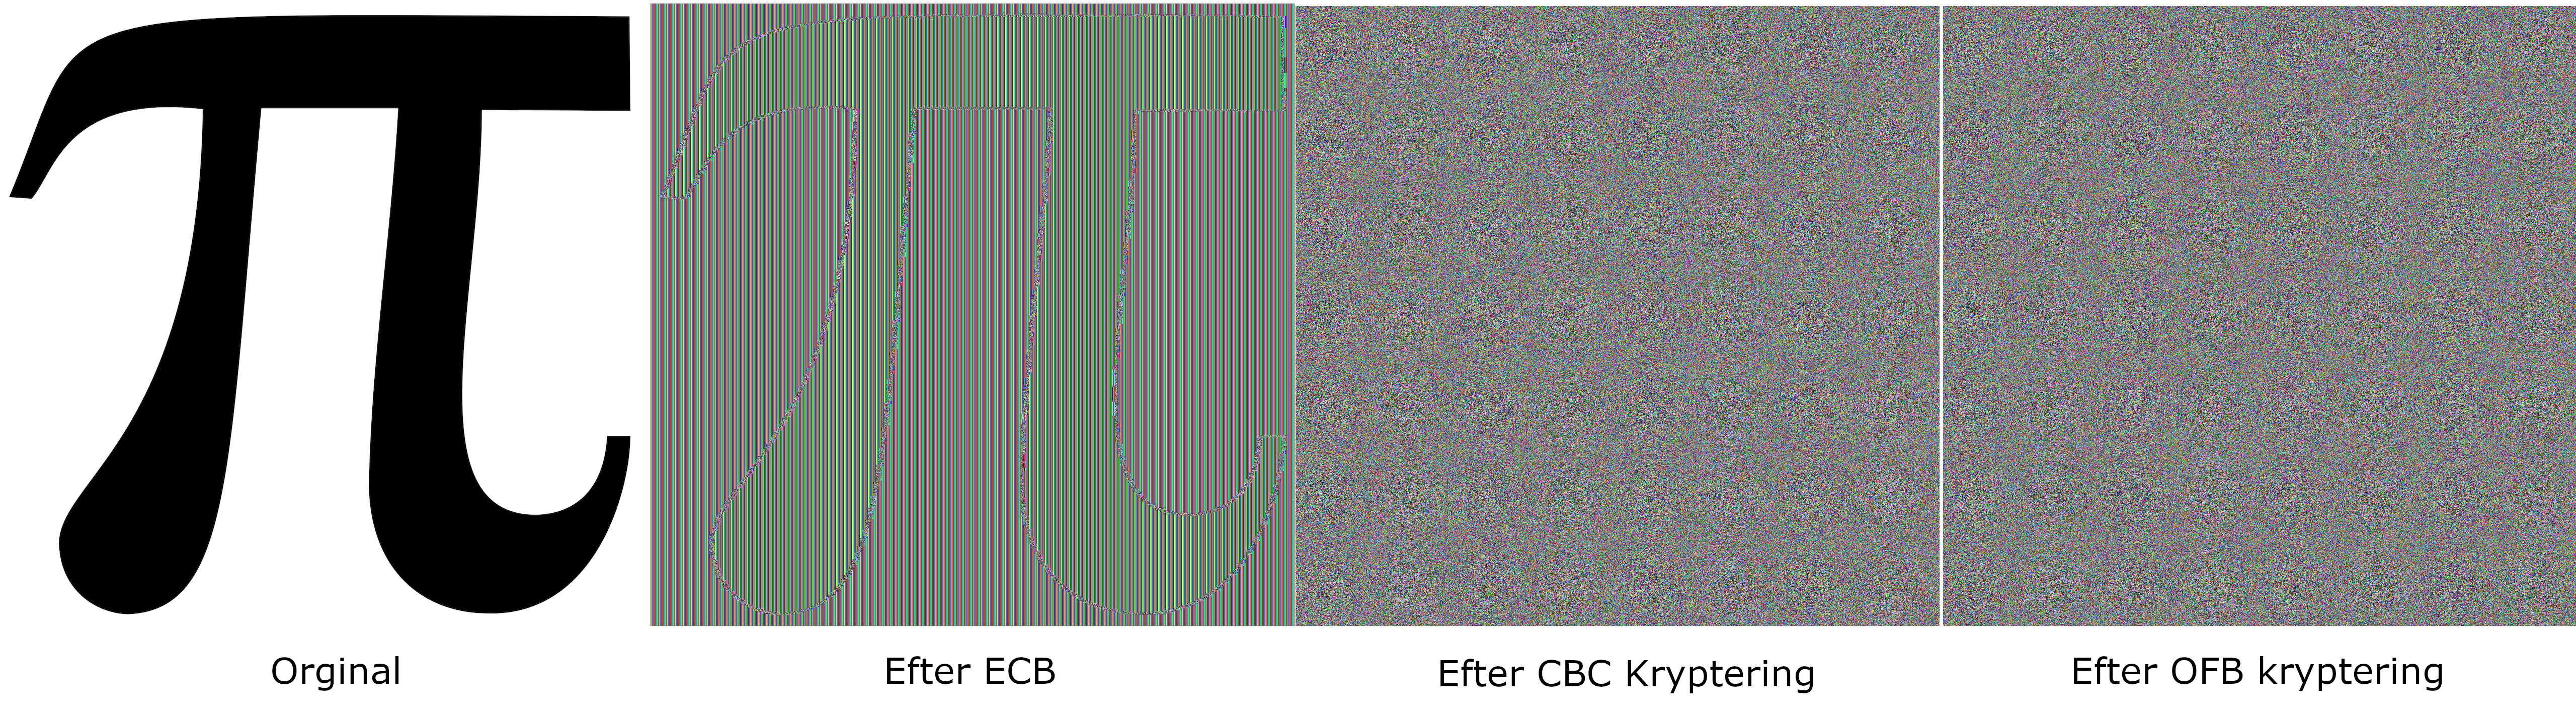
\includegraphics[width=0.8\textwidth]{summarie-tp-background.png}
    \caption{\acrshort{aes} krypterings test (\acrshort{ecb}, \acrshort{cbc}, \acrshort{ofb})}
    \label{fig:aes-krypterings-test}
\end{figure}
